% THIS IS SIGPROC-SP.TEX - VERSION 3.1
% WORKS WITH V3.2SP OF ACM_PROC_ARTICLE-SP.CLS
% APRIL 2009
%
% It is an example file showing how to use the 'acm_proc_article-sp.cls' V3.2SP
% LaTeX2e document class file for Conference Proceedings submissions.
% ----------------------------------------------------------------------------------------------------------------
% This .tex file (and associated .cls V3.2SP) *DOES NOT* produce:
%       1) The Permission Statement
%       2) The Conference (location) Info information
%       3) The Copyright Line with ACM data
%       4) Page numbering
% ---------------------------------------------------------------------------------------------------------------
% It is an example which *does* use the .bib file (from which the .bbl file
% is produced).
% REMEMBER HOWEVER: After having produced the .bbl file,
% and prior to final submission,
% you need to 'insert'  your .bbl file into your source .tex file so as to provide
% ONE 'self-contained' source file.
%
% Questions regarding SIGS should be sent to
% Adrienne Griscti ---> griscti@acm.org
%
% Questions/suggestions regarding the guidelines, .tex and .cls files, etc. to
% Gerald Murray ---> murray@hq.acm.org
%
% For tracking purposes - this is V3.1SP - APRIL 2009

\documentclass{acm_proc_article-sp}

\usepackage{url} % for \url
\usepackage{textcomp} % for ®,©,etc.

\begin{document}

\title{USB in a microkernel based operating system}
\subtitle{[Extended Abstract]}
%
% You need the command \numberofauthors to handle the 'placement
% and alignment' of the authors beneath the title.
%
% For aesthetic reasons, we recommend 'three authors at a time'
% i.e. three 'name/affiliation blocks' be placed beneath the title.
%
% NOTE: You are NOT restricted in how many 'rows' of
% "name/affiliations" may appear. We just ask that you restrict
% the number of 'columns' to three.
%
% Because of the available 'opening page real-estate'
% we ask you to refrain from putting more than six authors
% (two rows with three columns) beneath the article title.
% More than six makes the first-page appear very cluttered indeed.
%
% Use the \alignauthor commands to handle the names
% and affiliations for an 'aesthetic maximum' of six authors.
% Add names, affiliations, addresses for
% the seventh etc. author(s) as the argument for the
% \additionalauthors command.
% These 'additional authors' will be output/set for you
% without further effort on your part as the last section in
% the body of your article BEFORE References or any Appendices.

\numberofauthors{2} %  in this sample file, there are a *total*
% of EIGHT authors. SIX appear on the 'first-page' (for formatting
% reasons) and the remaining two appear in the \additionalauthors section.
%
\author{
% You can go ahead and credit any number of authors here,
% e.g. one 'row of three' or two rows (consisting of one row of three
% and a second row of one, two or three).
%
% The command \alignauthor (no curly braces needed) should
% precede each author name, affiliation/snail-mail address and
% e-mail address. Additionally, tag each line of
% affiliation/address with \affaddr, and tag the
% e-mail address with \email.
%
% 1st. author
\alignauthor
Daniel Mierswa\\
       \affaddr{RheinMain University of Applied Sciences}\\
       \affaddr{Erlenweg 22}\\
       \affaddr{Taunusstein, Germany}\\
       \email{impulze@impulze.org}
% 2nd. author
\alignauthor
Daniel Tkocz\\
       \affaddr{RheinMain University of Applied Sciences}\\
       \affaddr{Schiffergasse 15}\\
       \affaddr{Wiesbaden, Germany}\\
       \email{daniel.tkocz42@gmail.com}
}
% There's nothing stopping you putting the seventh, eighth, etc.
% author on the opening page (as the 'third row') but we ask,
% for aesthetic reasons that you place these 'additional authors'
% in the \additional authors block, viz.
%\additionalauthors{Additional authors: John Smith (The Th{\o}rv{\"a}ld Group,
%email: {\texttt{jsmith@affiliation.org}}) and Julius P.~Kumquat
%(The Kumquat Consortium, email: {\texttt{jpkumquat@consortium.net}}).}
%\date{30 July 1999}
% Just remember to make sure that the TOTAL number of authors
% is the number that will appear on the first page PLUS the
% number that will appear in the \additionalauthors section.

\maketitle
\begin{abstract}
This paper provides an introduction in using USB in a microkernel operating system.
This paper also contains a small introduction in USB and microkernels for better understanding.
Problems that might occur are described and solutions are presented.
%This paper provides a sample of a \LaTeX\ document which conforms to
%the formatting guidelines for ACM SIG Proceedings.
%It complements the document \textit{Author's Guide to Preparing
%ACM SIG Proceedings Using \LaTeX$2_\epsilon$\ and Bib\TeX}. This
%source file has been written with the intention of being
%compiled under \LaTeX$2_\epsilon$\ and BibTeX.

%The developers have tried to include every imaginable sort
%of ``bells and whistles", such as a subtitle, footnotes on
%title, subtitle and authors, as well as in the text, and
%every optional component (e.g. Acknowledgments, Additional
%Authors, Appendices), not to mention examples of
%equations, theorems, tables and figures.

%To make best use of this sample document, run it through \LaTeX\
%and BibTeX, and compare this source code with the printed
%output produced by the dvi file.
\end{abstract}

% A category with the (minimum) three required fields
%\category{H.4}{Information Systems Applications}{Miscellaneous}
%A category including the fourth, optional field follows...
%\category{D.2.8}{Software Engineering}{Metrics}[complexity measures, performance measures]

%\terms{Theory}

\keywords{USB, microkernel, data sharing, driver development}% NOT required for Proceedings
\section{Introduction}
When the market for personal computers started to open up, programmers all over the world
started developing operating systems.
Some operating systems (e.g. UNIX) were using monolithic kernels, so a lot of code
was working in kernel mode.
Developers saw problems with this architecture and started the counter movement using microkernel
based operating systems.
Those kernels have small code footprint and pass messages to underlying services which facilitate
the hardware for programmers.
In the late 1990s microkernel development had its peak and todays work with microkernels is mostly
based on the architectures of this era.

In 1996, the Universal Serial Bus (USB) was developed.
USB was an attempt to standardize communication components of computer peripherals and
the protocols involved.
The underlying communication bus is shared amongst devices and poses a problem in a microkernel based
operating system due to the separation of functionality in tasks.

This paper presents a design, which will show how to support USB in microkernel based operating systems.
In sections \ref{sec:usb} and \ref{sec:microkernel}, the relevant parts of USB and microkernels are described
to understand the terminology used in this paper.
Section \ref{sec:both} describes problems that may occur in a microkernel environment using USB and the following
section \ref{sec:serv} will provide a design which is capable of solving those problems.

\section{USB}
Universal Serial Bus (USB) is a serial bus.
With USB it is possible to connect a lot of different types of devices to a host.
Today, the most common USB devices are keyboards and mice.
But also external storage, mobile phones and gadgets like a small rocket launcher can be connected to a host by USB.
USB supports hot plugging of USB devices.
That means connecting, disconnecting and detecting a USB device to/from a running host.

\subsection{Hardware}
There is a large amount of different USB connectors (Type A, Type B, Mini A, Mini AB, Mini B, Micro AB, Micro B, Type C \cite{usborg}).
They vary in size, profile, durability, compatibility and usability \cite{dowell}.
The pins used in USB 1.x/2.0 in each of the connectors are nearly the same.

\begin{table}
\centering
\caption{USB 1.x/2.0 standard pinout}
\begin{tabular}{|l|l|l|l|} \hline
Pin & Name & Wire color & Description\\ \hline
1 & $V_{BUS}$ & Red (or orange) & + 5 V\\ \hline
2 & D- & White (or gold) & Data-\\ \hline
3 & D+ & Green & Data+\\ \hline
4 & GND & Black (or blue) & Ground\\ \hline
\end{tabular}
\end{table}

\begin{table}
\centering
\caption{USB 1.x/2.0 mini/micro pinout}
\begin{tabular}{|l|l|l|l|} \hline
Pin & Name & Wire color & Description\\ \hline
1 & $V_{BUS}$ & Red & + 5 V\\ \hline
2 & D- & White & Data-\\ \hline
3 & D+ & Green & Data+\\ \hline
4 & ID &  & Detect which connector is connected\\ \hline
5 & GND & Black & Ground\\ \hline
\end{tabular}
\end{table}

Only USB 3.x varies a lot. But some USB 3.0 connectors are backward compatible.
$V_{BUS}$ and GND supply the connected device with power varying (depending on specification) from 0.5 A to 3 A at 5 V in general \cite{beyond}.
The wires in a USB cable are twisted to reduce noise.
The communication in USB 1.x/2.0 is half duplex, USB 3.x is full duplex.
Depending on the USB version the transfer rate is 1.5 Mbit/s up to 10 Gbit/s.
USB 2.0 has a transfer rate of 480 Mbit/s \cite{beyond}.

\subsection{Software} %http://www.beyondlogic.org/usbnutshell/usb1.shtml
\subsubsection{Device Descriptor} %http://www.usb.org/developers
The device descriptor specifies a couple of informations about a device.
All information can be printed on the console of a Linux system by entering \emph{lsusb -v} in a terminal.
The device descriptor is only one descriptor from a small group.
This group consists of configuration descriptors -- which describe how much power the device needs and
which power mode is used (sleep, self powered, etc.) -- ,
the endpoint descriptor -- described later -- , the interface endpoint -- which bundles a group of
endpoint descriptors -- and string descriptors -- which contain a single string instead of hex numbers \cite{beyond}.

\begin{description}
\item[USB version]
The device descriptor also holds the used USB version.
By manipulating this field in the device descriptor, a USB 2.0 device can connect to a host as USB 1.1 device \cite{beyond}.

\item[Device class]
Class codes are used to specify the functionality of a device.
They are communicated to the host to determine if the device is supported and if so decide which driver should be used for it.
For example, a device identifying itself with the class code $0E_h$ should be treated as a webcam providing a video signal.
By way of comparison, a device sending $03_h$ should be treated as a human interface device (keyboard, mouse, etc.).
If no device specific driver exists, a generic driver will try to control the device.
If the manufacturer thinks none of the device classes matches the functionality, the manufacturer can decide to use a
vendor specific class: $FF_h$ \cite{axel}.
This might be a good idea for a USB rocket launcher.

\item[Device subclass]
The subclass specifies in detail what kind of device it is.

\item[Device protocol]
The protocol field defines a protocol which should be used to communicate with it.

\item [IDs \& numbers]
The device descriptor contains a vendor id to identify the manufacturer of a device.
To identify the product of a manufacturer, a product id is used.
A device release number and a serial number can be set additionally to specify the
hardware configuration.

\end{description}

\subsection{Endpoints}
Endpoints are used for communication.
Each communication is directed to a specific endpoint.
A device/host might have multiple endpoints for different purposes.
There are four different types of endpoints.
The integrity of a transfer is secured by a CRC sum for each endpoint.
To end a transfer, each message needs to be acknowledged except those from interrupt endpoints.
Endpoints are configured in an endpoint descriptor.
In general the communicated data can be split in three parts: \cite{beyond}
\begin{itemize}
\item Token Packet
\item Data Packet
\item Handshake Packet
\end{itemize}
Token packets specify the direction of the communication relative to the host.
IN means, the host receives data from the device, OUT means the host sends data to the device.\\
Data packets contain the data.
The passive side of the communication can send a STALL or not respond within a few milliseconds
\cite{beyond}.

\begin{figure}
\centering
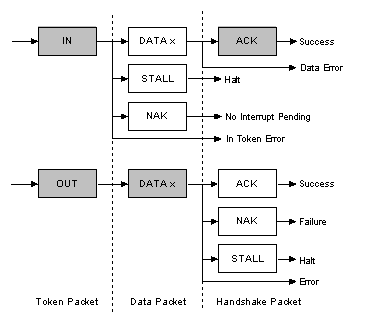
\includegraphics[width=0.4\textwidth]{interrupttransfer.png}
\label{fig:interrupttransfer}
\caption{Protocol of an interrupt transfer \cite{beyond}}
\end{figure}

\begin{description}
\item[Control endpoint]
Control endpoints are applied for control transfers and device configuration.
With them the device is configured.
Every device has a control endpoint (endpoint zero).

\item[Bulk endpoint]
Bulk endpoints are used for bulk transfers.
These non-time-critical transfers are applied for transferring large data
in read/write operations on external storage devices.

\item[Isochronous endpoint]
Isochronous endpoints are used for isochronous transfers.
Isochronous transfers are used if a specific transfer rate is required.

\item[Interrupt endpoint]
Interrupt endpoints are used for interrupt transfers.
Surprisingly this endpoint does not really work with interrupts in USB 2.0 or earlier versions.
Interrupt endpoints are polled each \emph{x} milliseconds.
They are often used for human interface devices.

\end{description}

\subsection{Packets}
For the whole communication packets are used.
Each message sent from an endpoint and received from an endpoint is based on a simple USB packet.
The packet overhead is only a few bytes depending on the used USB version.
The type of a packet determines what kind of data it contains.

\begin{description}
\item[Sync]
All packets start with a sync field.
This field is used to synchronize the timing of transmitter and receiver.

\item[PID]
To specify the content of a packet each sync field of a packet is followed by a PID field.
It contains a 4 bit information about the content.
To ensure integrity, the PID field contains twice the information to detect bit errors.

\item[ADDR]
The ADDR field specifies a device to communicate with.

\item[ENDP]
The ENDP field specifies an endpoint which should receive the packet.
Other Endpoints will not notice the packet at all.

\item[Data]
The data field contains up to 1 KB of custom data \cite{beyond}.

\item [CRC]
The CRC field contains a CRC sum of the data field \emph{only} to ensure integrity of the data.

\item[EOP]
The EOP field indicates the end of the package and is always the last in field in each package.

\end{description}

\section{Microkernel}
\label{sec:microkernel}
A microkernel ($\mu$-kernel) as opposed to a monolithic kernel has fewer code running in
supervisor mode (kernel mode).
\begin{figure}
\centering
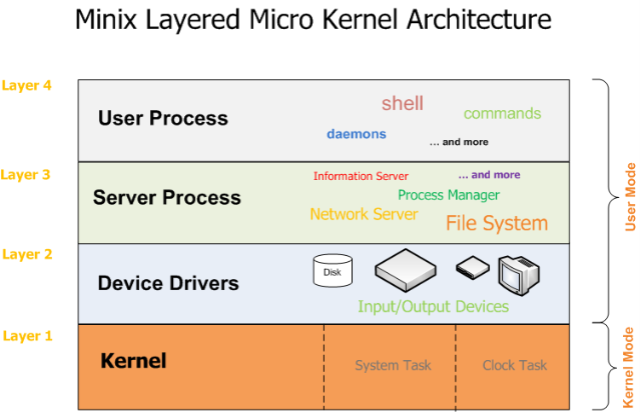
\includegraphics[width=0.4\textwidth]{minixinternalstructure.png}
\label{fig:minixmicarch}
\caption{The microkernel architecture as provided by Minix \cite{minix}}
\end{figure}
The architecture of microkernel based operating systems separates basic
hardware functionality from other layers of hardware access (as seen in Figure \ref{fig:minixmicarch}).
The modularization, if strictly executed, makes it easier for developers to support new
platforms, since they only have to port the machine-dependent code for basic hardware functionality \cite{black92}.
The code for system specific functionality (services) runs in user mode and as such
is not capable of interfering directly with hardware.
This demonstrates a challenge for driver developers and requires a well-defined kernel API.
Due to the separation and indirection, it is believed that microkernels cannot perform as fast as
monolithic kernels.
However, most of the performance issues of first generation microkernels were based on poor design
and faulty implementations \cite{p237-liedtke}.
Furthermore, device drivers implemented as services on microkernel operating systems can achieve
almost the same performance as monolithic drivers \cite{uldd}.

\subsection{Generations}
The idea of a microkernel was introduced in the late 1980s, however, at this point Unix \cite{unix}
was already widely used and adopted.
The concepts of Unix worked good enough around that time and BSD \cite{bsd} adoption of Unix started
the era of big kernels through adding filesystems and a complete TCP/IP stack. %[wiki]
The amount of code in kernels grew fast and with each new code fragment, the possibility of
freezing a system because of a faulty driver implementation increased.
Supporters of microkernel based operating systems argued that user-level implemented TCP/IP drivers
would simply restart the driver and leave the other OS functionality undamaged.
The Mach \cite{mach} microkernel was developed as a replacement to the mentioned BSD Unix.
It was developed from 1985 to the mid 90s at Carnegie Mellon University and is considered to be
the system that defines the first generation of microkernels.

Mach's external pager \cite{p70liedtke} manages physical and virtual memory in a way that allows
user-level code to map files and databases into their address space without using the filesystem
driver.
It also allows the usage of multiple systems simultaneously.
Another early idea was to implement Interrupt handling via Inter Process Communication (IPC).
IPC is the core component of any microkernel based operating system.
User-level servers can send/receive messages to/from the kernel or other user-level servers
through the kernel.
As one can see the implementation of the communication protocol is a bottleneck and optimization
is necessary to meet the requirements of todays applications.
Analysis of performance problems \cite{p70liedtke} showed that user-kernel-mode switches, address-space
switches and memory penalties also contributed to a bad performance.

In the mid 90s, development of new microkernels started.
They were written from scratch rather than evolving from the present monolithic kernels.
One of them was L4 \cite{l4}.
L4 has three abstraction layers: address spaces, threads and IPC.
Based on tests on a 486-DX5 machine, the L4 microkernel RPC was twice as fast as a UNIX system call
and 20 times faster than first generation IPC \cite{p70liedtke}.
The address space concept removed another limitation of first generation microkernels.
Basically it allows to construct address spaces recursively outside the kernel.
Memory management concepts used in the L4 kernel interface were an extension of the external
pager mechanisms presented in Mach kernels.

\section{USB in Microkernels}
\label{sec:both}
Earlier we presented the basic architecture of USB and how communication works on the serial bus.
In the previous chapter we've seen that microkernels are capable of accessing shared resources
(e.g. a bus) through APIs.
The obvious simple approach to support USB in a microkernel based operating system would be to provide
a service for the interaction with the Host Controller (HC) and let USB device drivers use the HC service.
If another USB device driver uses the HC service the USB Request Block (URB) coming from this device
driver would be blocked or queued.
This approach would work in a simple 1-to-1 relation when an operating system would just interact
with one USB device.
In real world scenarios however, we often face situations where one application (client) uses one or more
devices (interfacing with one or more device drivers), several applications use one or more devices or
devices communicating with each other (data transfer between mass-storage devices).
A simple ''blocking'' approach does not suffice and another component has to be provided to create a working
environment for USB device drivers.
It has to
\begin{itemize}
\item Create URBs based on certain scheduling parameters to avoid blocking
\item Fragment data so devices can be polled during huge data transfers
\item Prevent unauthorized bus access by other drivers
\end{itemize}
In this paper we try to present a separated USB service which will encapsulate this functionality.

\section{USB service}
\label{sec:serv}
We will look at the Linux USB driver architecture to get an understanding of how to separate concerns
in the handling of the USB protocol and introduce terms we will be using when describing the design
of the USB service.
\begin{figure}
\centering
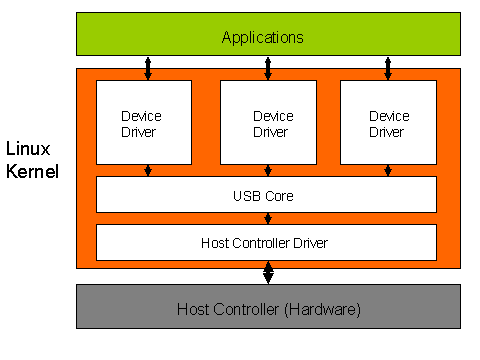
\includegraphics[width=0.4\textwidth]{usblinux.png}
\label{fig:usblinux}
\caption{Main components of the Linux USB driver}
\end{figure}
Figure \ref{fig:usblinux} shows how the operating system USB functionality can be split up into
major components.
The 3 components are:
\begin{itemize}
\item Driver for the Host Controller
\item USBCore support library
\item Drivers for USB devices
\end{itemize}
The Host Controller is the physical component which provides raw hardware access to devices.
The USBCore library is used to abstract functionality of the Host Controller without knowing
the details of the platform like handling interrupts, memory access and configuration.
An interface is provided for device drivers to manage memory and transfer data.
In addition, it provides the URB for the specific implementation and ways to communicate them.
Specific drivers for USB devices can use this library to access hardware and manage data flow.

An USB service would have to implement the USBCore functionality, so specific userspace
USB drivers can be implemented without wrestling with too many problems.
If we consider the 3 functionalities to provide a working USB environment, we will see the 2
main problems: deciding which URBs to send and authorize access.
Not providing a solution to either one of these problems could result in data loss,
data corruption or even broken hardware.
We can solve these problems by providing a queue for each driver, which will hold the URBs
for this driver and capability based access control.

\subsection{Scheduling}
Looking at URBs in a queue and deciding which URB to pick and send to the bus is called
scheduling.
While there are scheduling algorithms in hardware which can even be configured \cite{chs-ERSA03},
we will not consider those in the solution provided, since it should be possible to implement
the design on any microkernel.
There are scheduling algorithms which decide based on the priority of a task (such as fixed
priority scheduling).
These are not very helpful in this scenario.
Every device driver should be handled equally and thus have the same priority.
If a system is statically configured and/or embedded one could argue that the priorities of
the system are known (e.g. URBs from human interaction devices have a higher priority than
mass storage URBs).
Since the execution time of the operation (transmitting an URB over the bus) should not change,
algorithms such as Shortest Job First (SJF) are not looked at in this solution.
If the URBs would be scheduled with a First In first Out (FIFO) scheduler, a faulty driver
or a long operation could block all other drivers from accessing the bus.
Instead, the service will have a round-robin approach and will check if any device has URBs
ready to be transmitted.
Scheduling of own work is done by the driver itself.
A mechanism is provided by the service to create a queue in the address space of the service.
This results in IPC between the service and device driver for every URB that is created by
the driver.
Another solution would be the isolation of the URB queue in the address space of the device
driver.
However, this results in an IPC, even if the device driver has nothing to transmit at the
time the service checks for ready URBs.

\subsection{Access control}
%TODO
One may not want to allow any application to access devices using USB.
One scenario might be that an external data storage is fully loaded by a low priority
task (e.g. writing log files) while a high priority task tries to access the device (e.g. storing
data during emergency shutdown), but can not due to the low priority task.
To handle such scenarios, access rights management is required.
Both mechanisms that will be introduced are reliable and represent an access matrix
for objects in domains.

\paragraph{Capabilities}
A mechanism to enforce access control is using capability lists.
Capability lists are \emph{object right pairs} which belong to a domain \emph{d}.
Every time an USB operation would try to access object \emph{o} in a domain \emph{d} (or application/task)
it would need a capability to do so.

\paragraph{Access Control List}
Access Control List (ACL) is another mechanism to enforce access control.
ACL is a list of \emph{domain right pairs} which are attached to an object \emph{o}.
In contrast, ACLs belong to an object \emph{o}.
If an application/task (domain \emph{d}) is trying to access object \emph{o}, it is checked
(in the ACL) if the operation is allowed for this application.

While ACLs can be isolated in the USB service and controlled easily via lookup tables,
capabilities can be stored in a task or application and be reused to reduce overhead.
We decided to use capabilities to grant access to applications to send URBs
via the USB library offered by the USB service.
Some operating systems like seL4 microkernel based ones \cite{sel4} use capabilities
and are therefore a good example of how capabilities can be used in a microkernel
environment.
In a capability based system the mere possession of a capability entitles
the application to send URBs and there is no need for the USB service to
check any rights during operations.
An owner of a device, probably the application which opens the device first,
is allowed to change USB capabilities in the system.
It may also exclusively block the device.
This may be relevant in USB adapters for terminals for example.
The owner may also specify a default capability which is given to any
application by default when opening the device.

\subsection{Architecture}
Users will access USB components via a service library API of the USB service.
In forwarding direction, the application uses the library to send specific data
over USB in which case the call is merely forwarded to the USB device driver
(e.g. keyboard, mouse, etc.).
The device driver will then create URBs and queue them in the device driver.
In figure \ref{fig:usbsched} you can see (in red) a periodic task of the USB service
which will check each device driver queue for URBs and put them on the host controller.
This will be done in a round robin fashion to prevent devices to spam URBs.
\begin{figure}
\centering
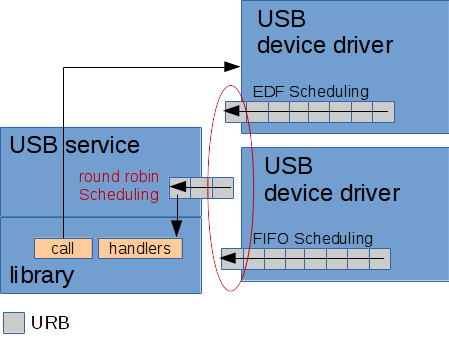
\includegraphics[width=0.5\textwidth]{usbsched.png}
\caption{Scheduling of the USB service}
\label{fig:usbsched}
\end{figure}
The device drivers will then create appropriate data structures and send them
to the USB service, which can then call appropriate installed handlers.
Those handlers may be setup by the application using the library to handle
asynchronous data transfers or they can be wrapped by the library internally
in order to simulate synchronous calls.
To allow different device drivers, an API has to be provided which must be implemented
by device drivers so that the service can send/receive URBs to/from the queue.

In order to gain access to USB devices an application uses the library
to open it.
It is then considered as owner of that device.
An operating system task may then use this ownership to change capabilities
for any accessing application.
If there is no such capability for an application, a default capability will
be granted which doesn't allow any operation for that application.
How those capabilities may actually look like in a real world application
is out of the scope of this paper.
An application could be identified by the process name or functionality.

\section{Conclusions}
While designing the USB service, it seemed the problems to be
solved are not specific to the domain of microkernels.
The solution presented in this paper designs a single task
that is responsible to grant access and manage data flow
of USB request blocks.
Therefore even the Linux device drivers can be ported
to microkernels by sending the URBs to the service and not to
the Linux kernel itself.

The USB service considers all device drivers and URBs to have
an equal priority which is not really real world applicable.
Future work should provide a parameter to the scheduling system
which gives the service a hint which URB queues to check
more often.
This would result in a scheduler that's no longer completely
fair, but which may be better suited for real time systems or
systems with lots of user interaction (keyboards, etc.).

\section{Acknowledgments}
We'd like to thank Daniel Ernst and Matthias Jurisch
of RheinMain University of Applied Science for their design proposal \cite{ernst}
which originated from the same ideas we have.
Besides very few specifics our approach is identical.

%
% The following two commands are all you need in the
% initial runs of your .tex file to
% produce the bibliography for the citations in your paper.
\bibliographystyle{abbrv}
\bibliography{sigproc-sp}
%\bibliography{sigproc}  % sigproc.bib is the name of the Bibliography in this case
% You must have a proper ".bib" file
%  and remember to run:
% latex bibtex latex latex
% to resolve all references
%
% ACM needs 'a single self-contained file'!
%
%APPENDICES are optional
\end{document}
